\documentclass[10pt,journal, twocolumn,letterpaper]{IEEEtran}
\IEEEoverridecommandlockouts    
\usepackage{fancyhdr}
\usepackage{graphics} % for pdf, bitmapped graphics files
\usepackage{amsmath}
\usepackage{amssymb}
\usepackage{graphicx}
% \usepackage{fixltx2e}
\usepackage{float}
\usepackage{placeins}
\usepackage{hyperref}
\usepackage[nameinlink]{cleveref}
%\usepackage{dblfloatfix}
\usepackage{flushend}
\usepackage{color,soul}
% \usepackage{todonotes}
\usepackage{mathtools}
\usepackage{url}
\usepackage{svg}
\DeclarePairedDelimiter\ceil{\lceil}{\rceil}
\hyphenation{op-tical net-works semi-conduc-tor}
\usepackage{dirtytalk}
\usepackage{gensymb}

\usepackage{caption}
\usepackage{subcaption}
\usepackage{todonotes}
\newcommand{\tdi}[1]{\todo[inline]{#1}}

\usepackage[acronym,toc,nomain]{glossaries}

\newacronym{ac}{AC}{Atmospheric Correction}
\newacronym{adcs}{ADCS}{Attitude Determination and Control System}
\newacronym{adgm}{ADGM}{Agile Decision-Guidance Method}
\newacronym{ai}{AI}{Artifical Intelligence}
\newacronym{ait}{AIT}{Assembly, Integration, and Testing}
\newacronym{aiv}{AIV}{Assembly, Integration, and Verification}
\newacronym{amos}{AMOS}{Centre for Autonomous Marine Operations and Systems}
\newacronym{aoi}{AoI}{Area of Interest}
\newacronym{api}{API}{Application Programing Interface}
\newacronym{apsco}{APSCO}{Asia-Pacific Space Cooperation Organization}
\newacronym{asv}{ASV}{Autonomous Surface Vehicle}
\newacronym{auv}{AUV}{Autonomous Underwater Vehicle}
\newacronym{aviris-ng}{AVIRIS-NG}{Airborne Visible-Infrared Imaging Spectrometer - Next Generation}

\newacronym{bbm}{BBM}{BreadBoard Model}
\newacronym{birds}{BIRDS}{Joint Global Multi-Nation BIRDS Satellite Project}
\newacronym{bob}{BOB}{Break-Out Board}
\newacronym{boussole}{BOUSSOLE}{buoy for the acquisition of a long-term optical time series}
\newacronym{bpr}{BPR}{Business Process Reengineering}
\newacronym{bssm}{BSSM}{Boardman's Soft Systems Engineering}

\newacronym{cad}{CAD}{Computer Aided Drafting}
\newacronym{calpoly}{CalPoly}{California Polytechnic State University}
\newacronym{can}{CAN}{Controller Area Network}
\newacronym{ccsds}{CCSDS}{Consultative Committee for Space Data Systems}

\newacronym{cdom}{CDOM}{Colored Dissolved Organic Matter}
\newacronym{cdr}{CDR}{Critical Design Review}
\newacronym{ce}{CE}{Concurrent Engineering}
\newacronym{chla}{Chl-a}{Chlorophyll-a ($\text{mg}/{\text{m}}^{-3}$)}
\newacronym{chl-a}{[Chl a]}{Chlorophyll-a concentration ($\text{mg}/{\text{m}}^{-3}$)}
\newacronym{ci}{CI}{Continuous Integration}
\newacronym{ciris}{CIRiS}{Center for Interdisciplinary Research in Space}
\newacronym{cli}{CLI}{Command Line Interface}
\newacronym{cmcc}{CMCC}{Coordinated Mission Control Center}
\newacronym{cmos}{CMOS}{complementary metal oxide semiconductor}
\newacronym{cots}{COTS}{Commercial-Off-The-Shelf}
\newacronym{covid}{COVID-19}{Coronavirus}
\newacronym{cps}{CPS}{Cyber-Physical Systems}
\newacronym{cpu}{CPU}{Central Processing Unit}
\newacronym{crm}{CRM}{CubeSat Reference Model}
\newacronym{cs}{CS}{Constituent System}
\newacronym{csp}{CSP}{Cubesat Space Protocol}
\newacronym{csrm}{CSRM}{CubeSat System Reference Model}
\newacronym{ctd}{CTD}{Conductivity for salinity, Temperature, and Depth for pressure of seawater}
\newacronym{cubesat}{CubeSat}{Cube Satellite}
\newacronym{czcs}{CZCS}{Coastal Zone Color Scanner}

\newacronym{de}{DE}{Digital Engineering}
\newacronym{dmc}{DMC}{Disaster Monitoring Constellation}
\newacronym{dod}{DoD}{Department of Defense}

\newacronym{eclipse}{ECLIPSE}{ECSS Compliant Toolset for Information and Projects Support of Enterprises in Space}
\newacronym{ecss}{ECSS}{European Cooperation for Space Standardization}
\newacronym{ecm}{ECM}{Enterprise Content Management}
\newacronym{egse}{EGSE}{Electrical Ground Support Equipment}
\newacronym{em}{EM}{Engineering Model}
\newacronym{eo}{EO}{Earth Observation}
\newacronym{eps}{EPS}{Electrical Power Unit}
\newacronym{esa}{ESA}{European Space Agency}
\newacronym{esd}{ESD}{ElectroStatic Discharge}
\newacronym{esf}{ESF}{Edge Spread Function}

\newacronym{fc}{FC}{Flight Computer}
\newacronym{fm}{FM}{Flight Model}
\newacronym{fmeca}{FMECA}{Failure Mode, Effects, and Criticality Analysis}
\newacronym{fov}{FOV}{Field-Of-View}
\newacronym{fpga}{FPGA}{Field Programmable Gate Array}
\newacronym{ft}{FT}{File Transfer}
\newacronym{fwhm}{FWHM}{Full-Width at Half-Maximum}

\newacronym{giop}{GIOP}{Generalized Inherent Optical Properties}
\newacronym{gps}{GPS}{Global Positioning System}
\newacronym{gpu}{GPU}{Graphics Processing Unit}
\newacronym{grd}{GRD}{Ground Resolution Distance}
\newacronym{gs}{GS}{Ground Station}
\newacronym{gsd}{GSD}{Ground Sampling Distance}
\newacronym{gnss}{GNSS}{global navigation satellite system}
\newacronym{gse}{GSE}{Ground Support Equipment}

\newacronym{hab}{HAB}{Harmful Algal Bloom}
\newacronym{hdr}{HDR}{High Data Rate}
\newacronym{hico}{HICO}{Hyperspectral Imager for the Coastal Ocean}
\newacronym{hil}{HIL}{Hardware-In-the-Loop}
\newacronym{hipp}{HIPP}{Hyperspectral Image Processing Pipeline}
\newacronym{hsi}{HSI}{Hypespectral Imager}
\newacronym{hplc}{HPLC}{High-Performance Liquid Chromatography}
\newacronym{hypso}{HYPSO}{HYPerspectral Small satellite for ocean Observation}
\newacronym{hw}{HW}{hardware}

\newacronym{icd}{ICD}{Interface Control Document}
\newacronym{ies}{IES}{Department of Electronic Systems}
\newacronym{imu}{IMU}{inertial measurement unit}
\newacronym{incose}{INCOSE}{International Council On Systems Engineering}
\newacronym{ioccg}{IOCCG}{International Ocean-Colour Coordinating Group}
\newacronym{iod}{IOD}{In-Orbit Demonstration}
\newacronym{iop}{IOP}{Inherent Optical Properties}
\newacronym{irl}{IRL}{Integration Readiness Level}
\newacronym{iso}{ISO}{International Standards Organization}
\newacronym{iss}{ISS}{International Space Station}
\newacronym{itk}{ITK}{Department of Engineering Cybernetics}
\newacronym{itu}{ITU}{International Telecommunication Union}

\newacronym{lasso}{Least Absolute Shrinkage and Selection Operator}{LASSO}
\newacronym{lba}{LBA}{Light Beam Attenuation}
\newacronym{ldr}{LDR}{Low Data Rate}
\newacronym{leo}{LEO}{Low-Earth Orbit}
\newacronym{lsf}{LSF}{Line Spread Function}

\newacronym{massive}{MASSIVE}{Mission-oriented Autonomous Systems with Small Satellites for Maritime Sensing, Surveillance and Communication}
\newacronym{mbse}{MBSE}{Model-Based Systems Engineering}
\newacronym{mcc}{MCC}{Mission Control Center}
\newacronym{mce}{MCE}{Model-Centric Engineering}
\newacronym{mcs}{MCS}{Mission Control System}
\newacronym{mdr}{MDR}{Mission Design Review}
\newacronym{measat}{MEASAT}{Malaysia East Asia Satellite}
\newacronym{meris}{MERIS}{Medium Resolution Imaging Spectrometer}
\newacronym{mgse}{MGSE}{Mechanical Ground Support Equipment}
\newacronym{mil}{MIL}{Model-In-the-Loop}
\newacronym{mit}{MIT}{Massachusetts Institute of Technology}
\newacronym{ml}{ML}{Machine Learning}
\newacronym{mm}{MM}{Mass Model}
\newacronym{moby}{MOBY}{Marine Optical BuoY}
\newacronym{moe}{MOE}{Measures of Effectiveness}
\newacronym{ms}{MS}{Mission Success}
\newacronym{mvp}{MVP}{Minimum Viable Product}

\newacronym{nasa}{NASA}{National Aeronautics and Space Administration}
\newacronym{nfr}{NFR}{Norsk Forskningsråd}
\newacronym{nifro}{NIFRO}{Norwegian Industrial Forum for Space Activities}
\newacronym{nir}{NIR}{Near-Infrared}
\newacronym{nn}{NN}{Neural Network}
\newacronym{nng}{NNG}{Nanomsg Next Generation}
\newacronym{nrc}{NRC}{Research Council of Norway}
\newacronym{nstp}{NSTP}{NASA Technical Standards Program}
\newacronym{ntnu}{NTNU}{Norwegian University of Science and Technology}
\newacronym{nuts}{NUTS}{NTNU Test Satellite}

\newacronym{obc}{OBC}{On-board Computer}
\newacronym{obdh}{OBDH}{On-Board Data Handling}
\newacronym{obip}{OBIP}{On-board Image Processing}
\newacronym{ogse}{OGSE}{Optical Ground Support Equipment}
\newacronym{omg}{OMG}{Object Management Group}
\newacronym{ooda}{OODA}{Observe-Orient-Decide-Act}
\newacronym{opu}{OPU}{On-board Processing Unit}
\newacronym{os}{OS}{Operating System}
\newacronym{otfp}{OTFP}{On-The-Fly Processing}

\newacronym{par}{PAR}{Participatory Action Research}
\newacronym{pbob}{picoBoB}{PicoZed + Break-out-Board}
\newacronym{pc}{PC}{Payload Controller}
\newacronym{pca}{PCA}{Principal Component Analysis}
\newacronym{pcb}{pcb}{Printed Circuit Board}
\newacronym{pdr}{PDR}{Preliminary Design Review}
\newacronym{pls}{PLS}{Partial Least Squares}
\newacronym{plsr}{PLSR}{Partial Least Squares Regression}
\newacronym{pm}{PM}{Project Management}
\newacronym{pmi}{PMI}{Project Management Institute}
\newacronym{pr}{PR}{Pull Request}
\newacronym{psf}{PSF}{Point Spread Function}
\newacronym{pslv}{PSLV}{Polar Satellite Launch Vehicle}
\newacronym{psu}{PSU}{Power Supply Unit}
\newacronym{ptc}{PTC}{Passive Thermal Control}

\newacronym{qaa}{QAA}{Quasi-Analytical Algorithm}
\newacronym{qm}{QM}{Qualification Model}

\newacronym{ram}{RAM}{Reliability, Availability, Maintainability}
\newacronym{rcn}{RCN}{Research Council of Norway}
\newacronym{rer}{RER}{Relative Edge Response}
\newacronym{rf}{RF}{Radio Frequency}
\newacronym{rgb}{RGB}{Red-Green-Blue}
\newacronym{rid}{RID}{Review Item Discrepancy}
\newacronym{rmse}{RMSE}{Root Mean Square Error}
\newacronym{rov}{ROV}{Remotely Operated Vehicle}
\newacronym{rt}{RT}{Radiative Transfer}

\newacronym{saa}{SAA}{Semi-Analytical Algorithm}
\newacronym{sba}{SBA}{Skylight-Blocked Approach}
\newacronym{sc}{s/c}{spacecraft}
\newacronym{sdo}{SDO}{Solar Dynamics Observatory}
\newacronym{sdr}{SDR}{Software Defined Radio}
\newacronym{se}{SE}{Systems Engineering}
\newacronym{see}{SEE}{Single Event Effect}
\newacronym{sem}{SEM}{Systems Engineering Management}
\newacronym{sme}{SME}{Small- and Medium-sized Enterprises}
\newacronym{serc}{SERC}{Space Engineering Research Center}
\newacronym{sil}{SIL}{Software-In-the-Loop}
\newacronym{sip}{SIP}{Software-Intensive Payload}
\newacronym{snr}{SNR}{Signal-to-Noise Ratio}
\newacronym{soa}{SOA}{Service-Oriented Architecture}
\newacronym{soc}{SoC}{System-on-Chip}
\newacronym{soho}{SOHO}{Solar and Heliospheric Observatory}
\newacronym{som}{SOM}{System-on-Module}
\newacronym{sos}{SoS}{System of Systems}
\newacronym{souies}{SOUIES}{Satellite Operations User Interface Enhancement Suite}
\newacronym{sp}{SP}{SpectroPhotometer}
\newacronym{spg4}{SPG4}{Simplified General Perturbations model 4 }
\newacronym{srl}{SRL}{System Readiness Level}
\newacronym{ssa}{SSA}{Space Situational Awareness}
\newacronym{ssh}{SSH}{Sea Surface Height}
\newacronym{ssm}{SSM}{Soft Systems Methodology}
\newacronym{sst}{SST}{Sea Surface Temperature}
\newacronym{sstl}{SSTL}{Surrey Satellite Technology Ltd.}
\newacronym{sswg}{SSWG}{Space Systems Working Group}
\newacronym{stk}{STK}{System Tool Kit}
\newacronym{sysml}{SysML}{System Modeling Language}
\newacronym{sw}{SW}{software}

\newacronym{tbd}{TBD}{To Be Determined}
\newacronym{tbc}{TBC}{To Be Confirmed}
\newacronym{tbr}{TBR}{To Be Resolved}
\newacronym{tle}{TLE}{Two-line Element Set}
\newacronym{toa}{ToA}{Top-of-Atmosphere}
\newacronym{trl}{TRL}{Technology Readiness Level}
\newacronym{tsm}{TSM}{Total Suspended Matter}

\newacronym{uav}{UAV}{Unmanned Aerial Vehicle}
\newacronym{ui}{UI}{User Intrerface}
\newacronym{un}{UN}{United Nations}
\newacronym{unis}{UNIS}{the University Centre in Svalbard}
\newacronym{usart}{USART}{Universal Synchronous and Asynchronous Receiver-Transmitter}
\newacronym{usv}{USV}{Unmanned Surface Vehicle}

\newacronym{vis}{VIS}{Visible}
\newacronym{vpn}{VPN}{Virtual Private Network}

\newacronym{xp}{XP}{Extreme Programming}


\begin{document}
\bstctlcite{IEEEexample:BSTcontrol}

%
% paper title
% Titles are generally capitalized except for words such as a, an, and, as,
% at, but, by, for, in, nor, of, on, or, the, to and up, which are usually
% not capitalized unless they are the first or last word of the title.
% Linebreaks \\ can be used within to get better formatting as desired.
% Do not put math or special symbols in the title.

% Define title
% \newcommand{\paperTitle}{Bare Demo of IEEEtran.cls for IEEE Journals}
% \newcommand{\paperTitle}{Hyperspectral Image Sharpening \\ of a Miniaturized Pushbroom Sensor}
\newcommand{\paperTitle}{Image Sharpening of a Miniaturized Earth Observing Hyperspectral Push-broom Sensor}



\newcommand{\green}{\color{green}}
\newcommand{\red}{\color{red}}
\newcommand{\black}{\color{black}}
\newcommand{\blue}{\color{blue}}

\title{\paperTitle}
%
%
% author names and IEEE memberships
% note positions of commas and nonbreaking spaces ( ~ ) LaTeX will not break
% a structure at a ~ so this keeps an author's name from being broken across
% two lines.
% use \thanks{} to gain access to the first footnote area
% a separate \thanks must be used for each paragraph as LaTeX2e's \thanks
% was not built to handle multiple paragraphs
%

\author{
        Sivert~Bakken,
        Joseph~L.~Garrett,
        Steven~Le~Moan,
        and~Tor~A.~Johansen% <-this % stops a space
\thanks{S. Bakken is with SINTEF Ocean.}
\thanks{J.~L.~Garrett and T.A.~Joahansen are with Department of Engineering Cybernetics, NTNU, Trondheim, Norway.}%
\thanks{S.~L.~Moan are with Department of Computer Science, NTNU, Gjøvik, Norway.}% <-this % stops a space
\thanks{Manuscript received TBD, 2023; revised TBD.}}

% note the % following the last \IEEEmembership and also \thanks - 
% these prevent an unwanted space from occurring between the last author name
% and the end of the author line. i.e., if you had this:
% 
% \author{....lastname \thanks{...} \thanks{...} }
%                     ^------------^------------^----Do not want these spaces!
%
% a space would be appended to the last name and could cause every name on that
% line to be shifted left slightly. This is one of those "LaTeX things". For
% instance, "\textbf{A} \textbf{B}" will typeset as "A B" not "AB". To get
% "AB" then you have to do: "\textbf{A}\textbf{B}"
% \thanks is no different in this regard, so shield the last } of each \thanks
% that ends a line with a % and do not let a space in before the next \thanks.
% Spaces after \IEEEmembership other than the last one are OK (and needed) as
% you are supposed to have spaces between the names. For what it is worth,
% this is a minor point as most people would not even notice if the said evil
% space somehow managed to creep in.

% The paper headers
\markboth{Journal of \LaTeX\ Class Files,~Vol.~14, No.~8, August~2015}%
{Shell \MakeLowercase{\textit{et al.}}: \paperTitle}
% The only time the second header will appear is for the odd numbered pages
% after the title page when using the twoside option.
% 
% *** Note that you probably will NOT want to include the author's ***
% *** name in the headers of peer review papers.                   ***
% You can use \ifCLASSOPTIONpeerreview for conditional compilation here if
% you desire.




% If you want to put a publisher's ID mark on the page you can do it like
% this:
%\IEEEpubid{0000--0000/00\$00.00~\copyright~2015 IEEE}
% Remember, if you use this you must call \IEEEpubidadjcol in the second
% column for its text to clear the IEEEpubid mark.



% use for special paper notices
%\IEEEspecialpapernotice{(Invited Paper)}




% make the title area
\maketitle

Here is a cite~\cite{Grotte2021}

% For peer review papers, you can put extra information on the cover
% page as needed:
% \ifCLASSOPTIONpeerreview
% \begin{center} \bfseries EDICS Category: 3-BBND \end{center}
% \fi
%
% For peerreview papers, this IEEEtran command inserts a page break and
% creates the second title. It will be ignored for other modes.

% Main Matter

\IEEEpeerreviewmaketitle
\glsresetall

%%%%%%%%%%%%%%%%%% MAIN MATTER














%%%%%%%%%%%%%%%%%% MAIN MATTER


% use section* for acknowledgment
\section*{Acknowledgment}


% The authors would like to thank... AMOS (223254), MASSIVE, Green-Platform, ELO-Hyp, HYPSCI,.... 
% NanoAvionics, KSAT, all master students, Frøya-folks, Ny-Ålesund folks, SOUIES BSc-group especially...

This work was supported by the Research Council of Norway through the Centre of Excellence funding scheme NTNU AMOS (grant no. 223254),  MASSIVE (grant no. 270959),  HYPSCI (grant no. 325961), and Green-Platform (grant no. 328724), NO Grants 2014 - 2021 under Project ELO-Hyp (contract no. 24/2020), the Norwegian Space Agency and the European Space Agency through PRODEX (no. 4000132515).
%
The authors would also like to thank the full \gls{hypso}-1 team, including all students that have been a part of the project, everyone contributing in the Frohavet and Ny-Ålesund campaigns, NanoAvionics for support with the satellite, and KSAT for extra downlink opportunities through the KSATlite network.

% Can use something like this to put references on a page
% by themselves when using endfloat and the captionsoff option.
\ifCLASSOPTIONcaptionsoff
  \newpage
\fi



% trigger a \newpage just before the given reference
% number - used to balance the columns on the last page
% adjust value as needed - may need to be readjusted if
% the document is modified later
%\IEEEtriggeratref{8}
% The "triggered" command can be changed if desired:
%\IEEEtriggercmd{\enlargethispage{-5in}}

% references section

% can use a bibliography generated by BibTeX as a .bbl file
% BibTeX documentation can be easily obtained at:
% http://mirror.ctan.org/biblio/bibtex/contrib/doc/
% The IEEEtran BibTeX style support page is at:
% http://www.michaelshell.org/tex/ieeetran/bibtex/
\bibliographystyle{IEEEtran}
% argument is your BibTeX string definitions and bibliography database(s)
% \bibliography{IEEEabrv,../bib/paper}
\bibliography{refs}
%
% <OR> manually copy in the resultant .bbl file
% set second argument of \begin to the number of references
% (used to reserve space for the reference number labels box)
% \begin{thebibliography}{1}

% \bibitem{IEEEhowto:kopka}
% H.~Kopka and P.~W. Daly, \emph{A Guide to \LaTeX}, 3rd~ed.\hskip 1em plus
%   0.5em minus 0.4em\relax Harlow, England: Addison-Wesley, 1999.

% \end{thebibliography}

%% Insert biographies here 

\begin{IEEEbiography}
[{
\includegraphics[width=1in,height=1.25in,clip,keepaspectratio]{fig/biography-photo/sivertba_headshot.jpg}}]{Sivert Bakken}
received the MSc degree in 2018 and the PhD degree in 2022, both in engineering Cybernetics, from the NTNU, Trondheim,
Norway. Currently working as postdoctoral Researcher at SINTEF Ocean for NTNU AMOS. Research focuses on how to utilize a small satellite with a hyperspectral imager as an intelligent agent in coordinated missions involving autonomous agents. 
\end{IEEEbiography}


\begin{IEEEbiography}[{
\includegraphics[width=1in,height=1.25in,clip,keepaspectratio]{fig/biography-photo/joe.png}}]{Joseph L. Garrett}
received a BSc in Physics and Mathematics from the Ohio State University in 2011 and a Ph.D. in Physics from the University of Maryland in 2017. He now studies hyperspectral imaging and image processing from satellites and drones as a researcher at NTNU. 
\end{IEEEbiography}

\begin{IEEEbiography}[{
\includegraphics[width=1in,height=1.25in,clip,keepaspectratio]{fig/biography-photo/stevenlemoan.jpeg}}]{Steven Le Moan}
received the Ph.D. degree in image processing from the University of Burgundy, France, in 2012. He then worked as a Postdoctoral Researcher at the Technical University of Darmstadt, Germany, and the Gjøvik University College, Norway. Until 2021, he was a Senior Lecturer in electronics, information and communication systems with Massey University, New Zealand. He is currently an Associate Professor of color imaging at the Norwegian University of Science and Technology, Gjøvik, Norway. His research interests include multi/hyperspectral image analysis, color science, and visual perception.
\end{IEEEbiography}


\begin{IEEEbiography}[{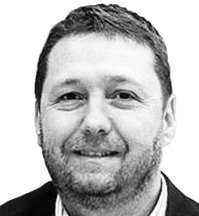
\includegraphics[width=1in,height=1.25in,clip,keepaspectratio]{fig/biography-photo/tor-arne-pic.jpg}}]{Tor A. Johansen}
received the MSc degree in 1989 
and the PhD degree in 1994, both in electrical and computer 
engineering, from the NTNU, Trondheim, Norway. From 1995 to 1997, he worked at SINTEF as a 
researcher before he was appointed Associated Professor at the 
NTNU in Trondheim in 1997 and  Professor in 2001. He has published several hundred articles 
in the areas of control, estimation and optimization with 
applications in the marine, aerospace, automotive, biomedical and process 
industries. In 2002 Johansen co-founded the company Marine 
Cybernetics AS where he was Vice President until 2008. Prof. 
Johansen received the 2006 Arch T. Colwell Merit Award of the SAE, 
and is currently a principal researcher within the Center of 
Excellence on Autonomous Marine Operations and Systems (NTNU-AMOS) 
and director of the Unmanned Aerial Vehicle Laboratory at NTNU and the 
SmallSat Laboratory at NTNU. He recently co-founded the spin-off 
companies Scout Drone Inspection, UBIQ Aerospace, Zeabuz and SentiSystems. 
\end{IEEEbiography}






% that's all folks
\end{document}


